\documentclass[12pt]{article}
\usepackage[english]{babel}
\usepackage{graphicx, amsmath, amsfonts, amsthm, mathtools, listings, color, caption, rotating, subfigure, fullpage, hyperref, textcomp, enumerate, float, listings, MnSymbol, wasysym}

\lstset{
	language=R,
	keywordstyle=\bfseries\ttfamily\color[rgb]{0,0,1},
	identifierstyle=\ttfamily,
	commentstyle=\color[rgb]{0.133,0.545,0.133},
	stringstyle=\ttfamily\color[rgb]{0.627,0.126,0.941},
	showstringspaces=false,
	basicstyle=\tiny,
	numberstyle=\scriptsize,
	numbers=left,
	stepnumber=1,
	numbersep=10pt,
	tabsize=2,
	breaklines=true,
	breakatwhitespace=false,
	aboveskip={1.5\baselineskip},
  columns=fixed,
  upquote=true,
  extendedchars=true,
}

\begin{document}
\begin{center}
STA250, Homework 2 \\
Christopher Aden\\
November 13, 2013\
\end{center}

\section*{A Bag of Little Bootstraps:}
Originally developed as an extension of the jackknife by Bradley Efron in 1979, the bootstrap is an indispensable statistical algorithm for acquiring standard errors (and confidence intervals) for estimators which have a difficult sampling distribution. The technique is a major advancement in statistical science, but it has suffered growing pains as the size of data has increased. In the ``big data'' world, the bootstrap, while it would be nice to have, requires a large number of resamplings of the original data of the same size. With sample sizes in the hundreds of millions, such a procedure breaks down--resampling many datasets of size ten million is expensive, difficult to store, and computing an estimator naively may be slow or impossible. The bag of little bootstraps (BLB) is a modern extension of the bootstrap that solves all such problems in a clever way.

First, it must be mentioned that the bag of little bootstraps is a method that only works on estimators that can be re-written in terms of a value and a count of the number of times that value is used. Examples of such estimators are means and proportions. BLB will not work if the estimator we want a standard error for cannot be computed using (value, count) pairs. Our algorithm goes as follows (taken from Minjie Fan's Lecture 8 notes, with modification):
\begin{enumerate}
  \item Let $\hat{F}$ denote the empirical probability distribution
  \item Select $s$ subsets of size $b$ from the full data. $b$ is taken without replacement.
  \item For each of the $s$ subsets ($j=1,\cdots,s$):
    \begin{itemize}
      \item Repeat the following steps $r$ times ($k=1,\cdots,r$):
        \begin{enumerate}
          \item Resample a bootstrap dataset $X_{j,k}^*$ of size $n$ from subset $j$.
          \item Compute and store the estimator $\hat{\theta}_{j,k}$
        \end{enumerate}
      \item Compute the bootstrap SE of $\hat{\theta}$ based on the $r$ bootstrap datasets for subset $j$.
    \end{itemize}
  \item Average the $s$ bootstrap SE's, $\xi_1^*,\cdots,\xi_s^*$ to obtain an estimate of $SD(\hat{\theta})$.
\end{enumerate}
The latter steps are done for us with code provided by Paul Baines. The bulk of the work that must be done is creating the $s$ subsets, saving them, and making all the $r$ little bootstraps from the larger $s$ ones, then computing the estimator in each case. This should give us the coefficients for the $r \cdot s$ datasets, which the provided code will then calculate the standard error of and average the bootstrap standard errors to get an estimate of the standard deviation. 

A couple tricks were done to increase the speed. The first trick was taking advantage of the description file that bigmemory provides for large arrays. The description file contains information about the number of rows, along with a nice hash table for the disk-based matrix. Taking the $s$ subsets would usually be a fairly intensive process for the disk I/O. This is because the subset operator is not super efficient at leverage the large matrix structure. Selecting rows naively will generally take quite awhile. Using the \verb+fmatch+ function in the package \verb+fastmatch+, this task was trivially fast, even on a matrix that took 15GB of disk storage! It's my personal opinion that hash tables are one of the best ways to speed up write-once, read-many (sorry for abusing the true use of the acronym WORM) operations like taking subsets from a largely, immutable dataset. This subsetting operation was done serially (though it could've been done in parallel on $s$ nodes), and each dataset was written as a native Rdata object. This made import and export of the object very easy and sidestepped the need to use read/write table functions, which are slow.

The $r \cdot s$ jobs were distributed across multiple nodes so that the job ran in parallel. For each of the $s$ samples from the full data, each of the $r$ threads read in the correct Rdata file, runs a linear model, then exports the coefficients to a file that incorporates the $r$ and $s$ values into the filename. This is to simplify looping over them when importing during aggregation.

The algorithm was generally pretty fast. The idea of randomly drawing $b$ distinct values from the original data set and drawing the counts from a multinomial is a pretty smart way to make an intractable problem a bit easier to solve. It was also easy to program. The only concern I have for the algorithm is the amount of I/O, having to generate a bunch of data sets. I believe my approach to be the most scalable, since I am not resampling the big dataset $r \cdot s$ times, but even still, the operation takes quite a bit of disk, writing files back and forth from disk to RAM. The standard errors seem to match up with the gold standard (the professor's estimates). The standard errors were all around $0.01$.
\begin{figure}[H] \center
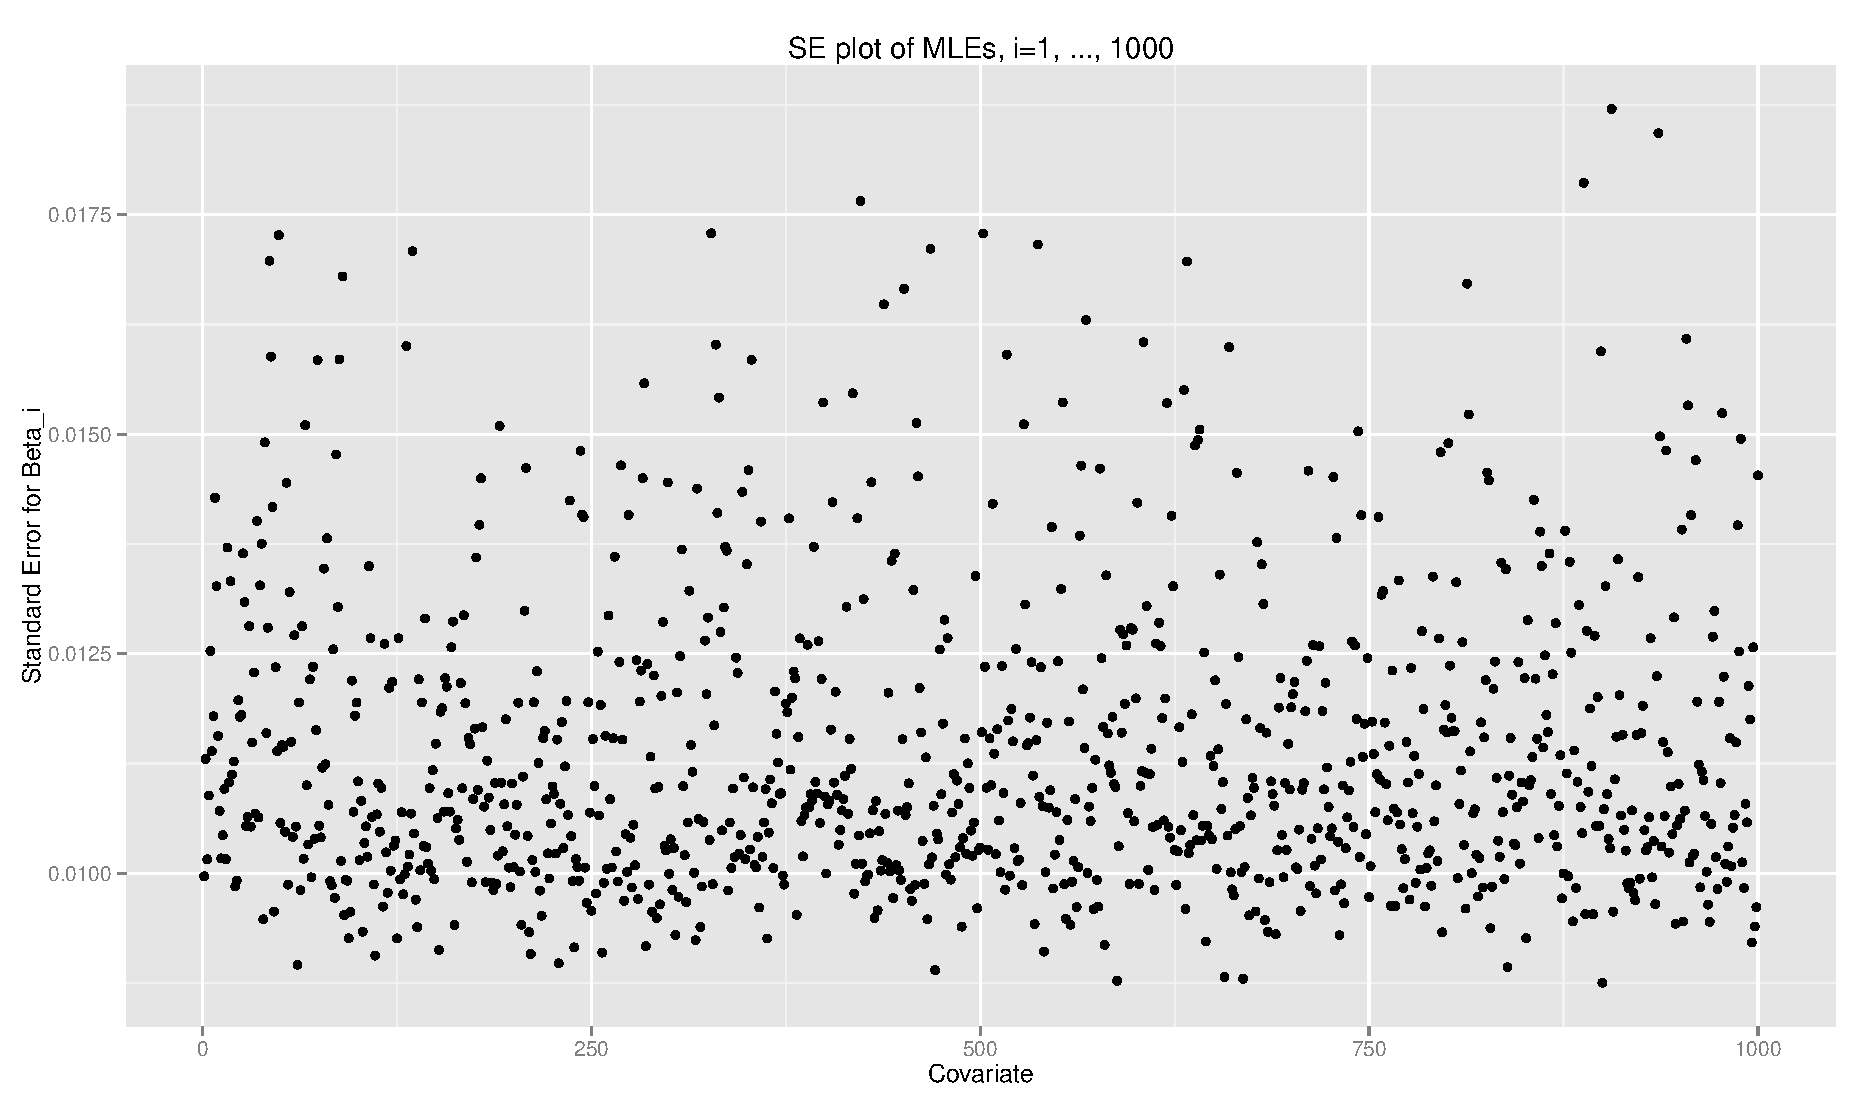
\includegraphics[scale=.55]{BLB/final/SD_plot.pdf}
\caption*{Standard Errors for each coefficient, $\beta_1, \dots, \beta_{1000}$.}
\end{figure}

\section*{MapReduce using Amazon's Elastic MapReduce (EMR)}
As far as theoretically difficult problems go, Bag of Little Bootstraps was the most difficult out of the three problems in the big data module. The MapReduce problem and the Hive problem are theoretically easy, yet technically a bit more difficult because of the newness of the technologies to statisticians. 

In this data, we have 180 million observed $(X,Y)$ pairs, split up into 100 files. The goal is to create a two-dimensional histogram by putting observations into bins of width $0.10$ and counting how many fall in each bin. In one dimension, a histogram will count the number of times a random variable, $X$ has observations in $(.10k < X \leq .10(k+1))$, where $k$ is some integer. In two dimensions, we need to count the number of times both variables, $X$ and $Y$, fall inside a box, so $(3.1415, 2.7182)$ would fall in the rectangle $X \in (3.1, 3.2), Y \in (2.7, 2.8)$. 

This task is well-suited to MapReduce, because we can individually determine what box each observation is going to fall into in parallel, then combine them all together, again using a high degree of parallelism. The algorithms are not particularly important in this case--Hadoop, the implementation of MapReduce we use, has abstracted a lot of the parallelism away from the users. The only things we need to worry about are writing the mapper function (determine the square of each observation) and the reducer function (count the number of observations per square).

In the mapper, we will read in the data from STDIN, one line at a time, extracting the pair. To each observation, we take the floor to the nearest tenth, as well as the ceiling to the nearest tenth. Doing this to each value of the pair gives us four values. I put these four values into a list, which I called my key. There was no particular reason for choosing a list for the four values, except that my key could then be just a single object. Since each line only has one pair, we can say that the number of times we saw any particular square on each line was just once. This made calculating the ``value'' (in Hadoop, the mapper always returns a key-value pair) trivial--just return $1$ as the value. The combination of the key (list of four floats, ordered ($x_{lo}, x_{hi}, y_{lo}, y_{hi}$), turned into a string) and the value (the integer $1$, coerced to string) were separated by tabs and printed to put it on STDOUT.

In between the mapper and the reducer, Hadoop is nice enough to sort my lines using the key. This means that my key-value pairs are all sorted with the smallest values of $x_{lo}$ coming first. This is convenient, because all my reducer needs to do is figure out how many times it sees a non-unique key. Every time the key is not unique, it can increment a counter, which keeps track of how many times it has seen that key. When a new key comes up, because the results from the mapper were sorted, we can be certain we will never again see that same key, and we are done counting that particular square. The result for that bin is sent to STDOUT, with each value of the bin dimensions and the final count separated by commas, similar to a CSV file. This proceeds until all key-value pairs from the mapper have been read by the reducer. 

Hadoop collects all results printed to STDOUT and saves them to a file. Given that many lines that had duplicate boxes are now compressed onto one line with a count of how many times they were duplicated, this output file is substantially smaller than the original data. The results are run through an R function that creates a two-dimensional histogram, using color to represent counts, similar to a heat map.

Hadoop replicates all the data into a virtual file system, stored within the local file system. This is necessary for Hadoop, which must break files into pieces and work on them all separately in small chunks in the name of parallelism. There is a Unix-like syntax for moving files between the local file system and Hadoop's file system. There are even functions on Amazon Web Services to easily move files from an S3 bucket into Hadoop's file system, which was the approach I took in this particular problem. This operation is fairly quick, given the size of the data involved in this problem.

There weren't any very difficult implementation choices to make. This style of problem is very well suited to MapReduce, so writing it was simple. The only real implementation choice to make was how to represent the key, as well as the functions needed to export the data in the reducer. I settled on a list of floats because, logically, it made sense to me to have the key be a single object, despite the key actually being a collection of four separate floats. It is possible I took a hit on speed from having to create a list in each of the 180 million lines, but the code ran quick enough (less than ten minutes) that I wasn't going to bother re-writing it to optimize for something that didn't matter. I would be curious to see how important the choice of data types for the key matter. The code is so simple, I doubt there's many changes I could make to speed it up. If 180 million observations in 10 minutes is too slow, other options would be either to scale up the number of compute instances (EMR stands for \emph{Elastic} MapReduce--scaling is very easy with Amazon Web Services), or write my MapReduce in the native Java instead of Python. Given how simple the code was, doing the latter might not be too difficult and would cut runtime substantially. 

I don't think porting the code to Java is worth it unless this operation is done more than a couple times a day. Refer to \url{xkcd.com/1205/} for more information about how much time to spend optimizing something.

\begin{figure}[H] \center
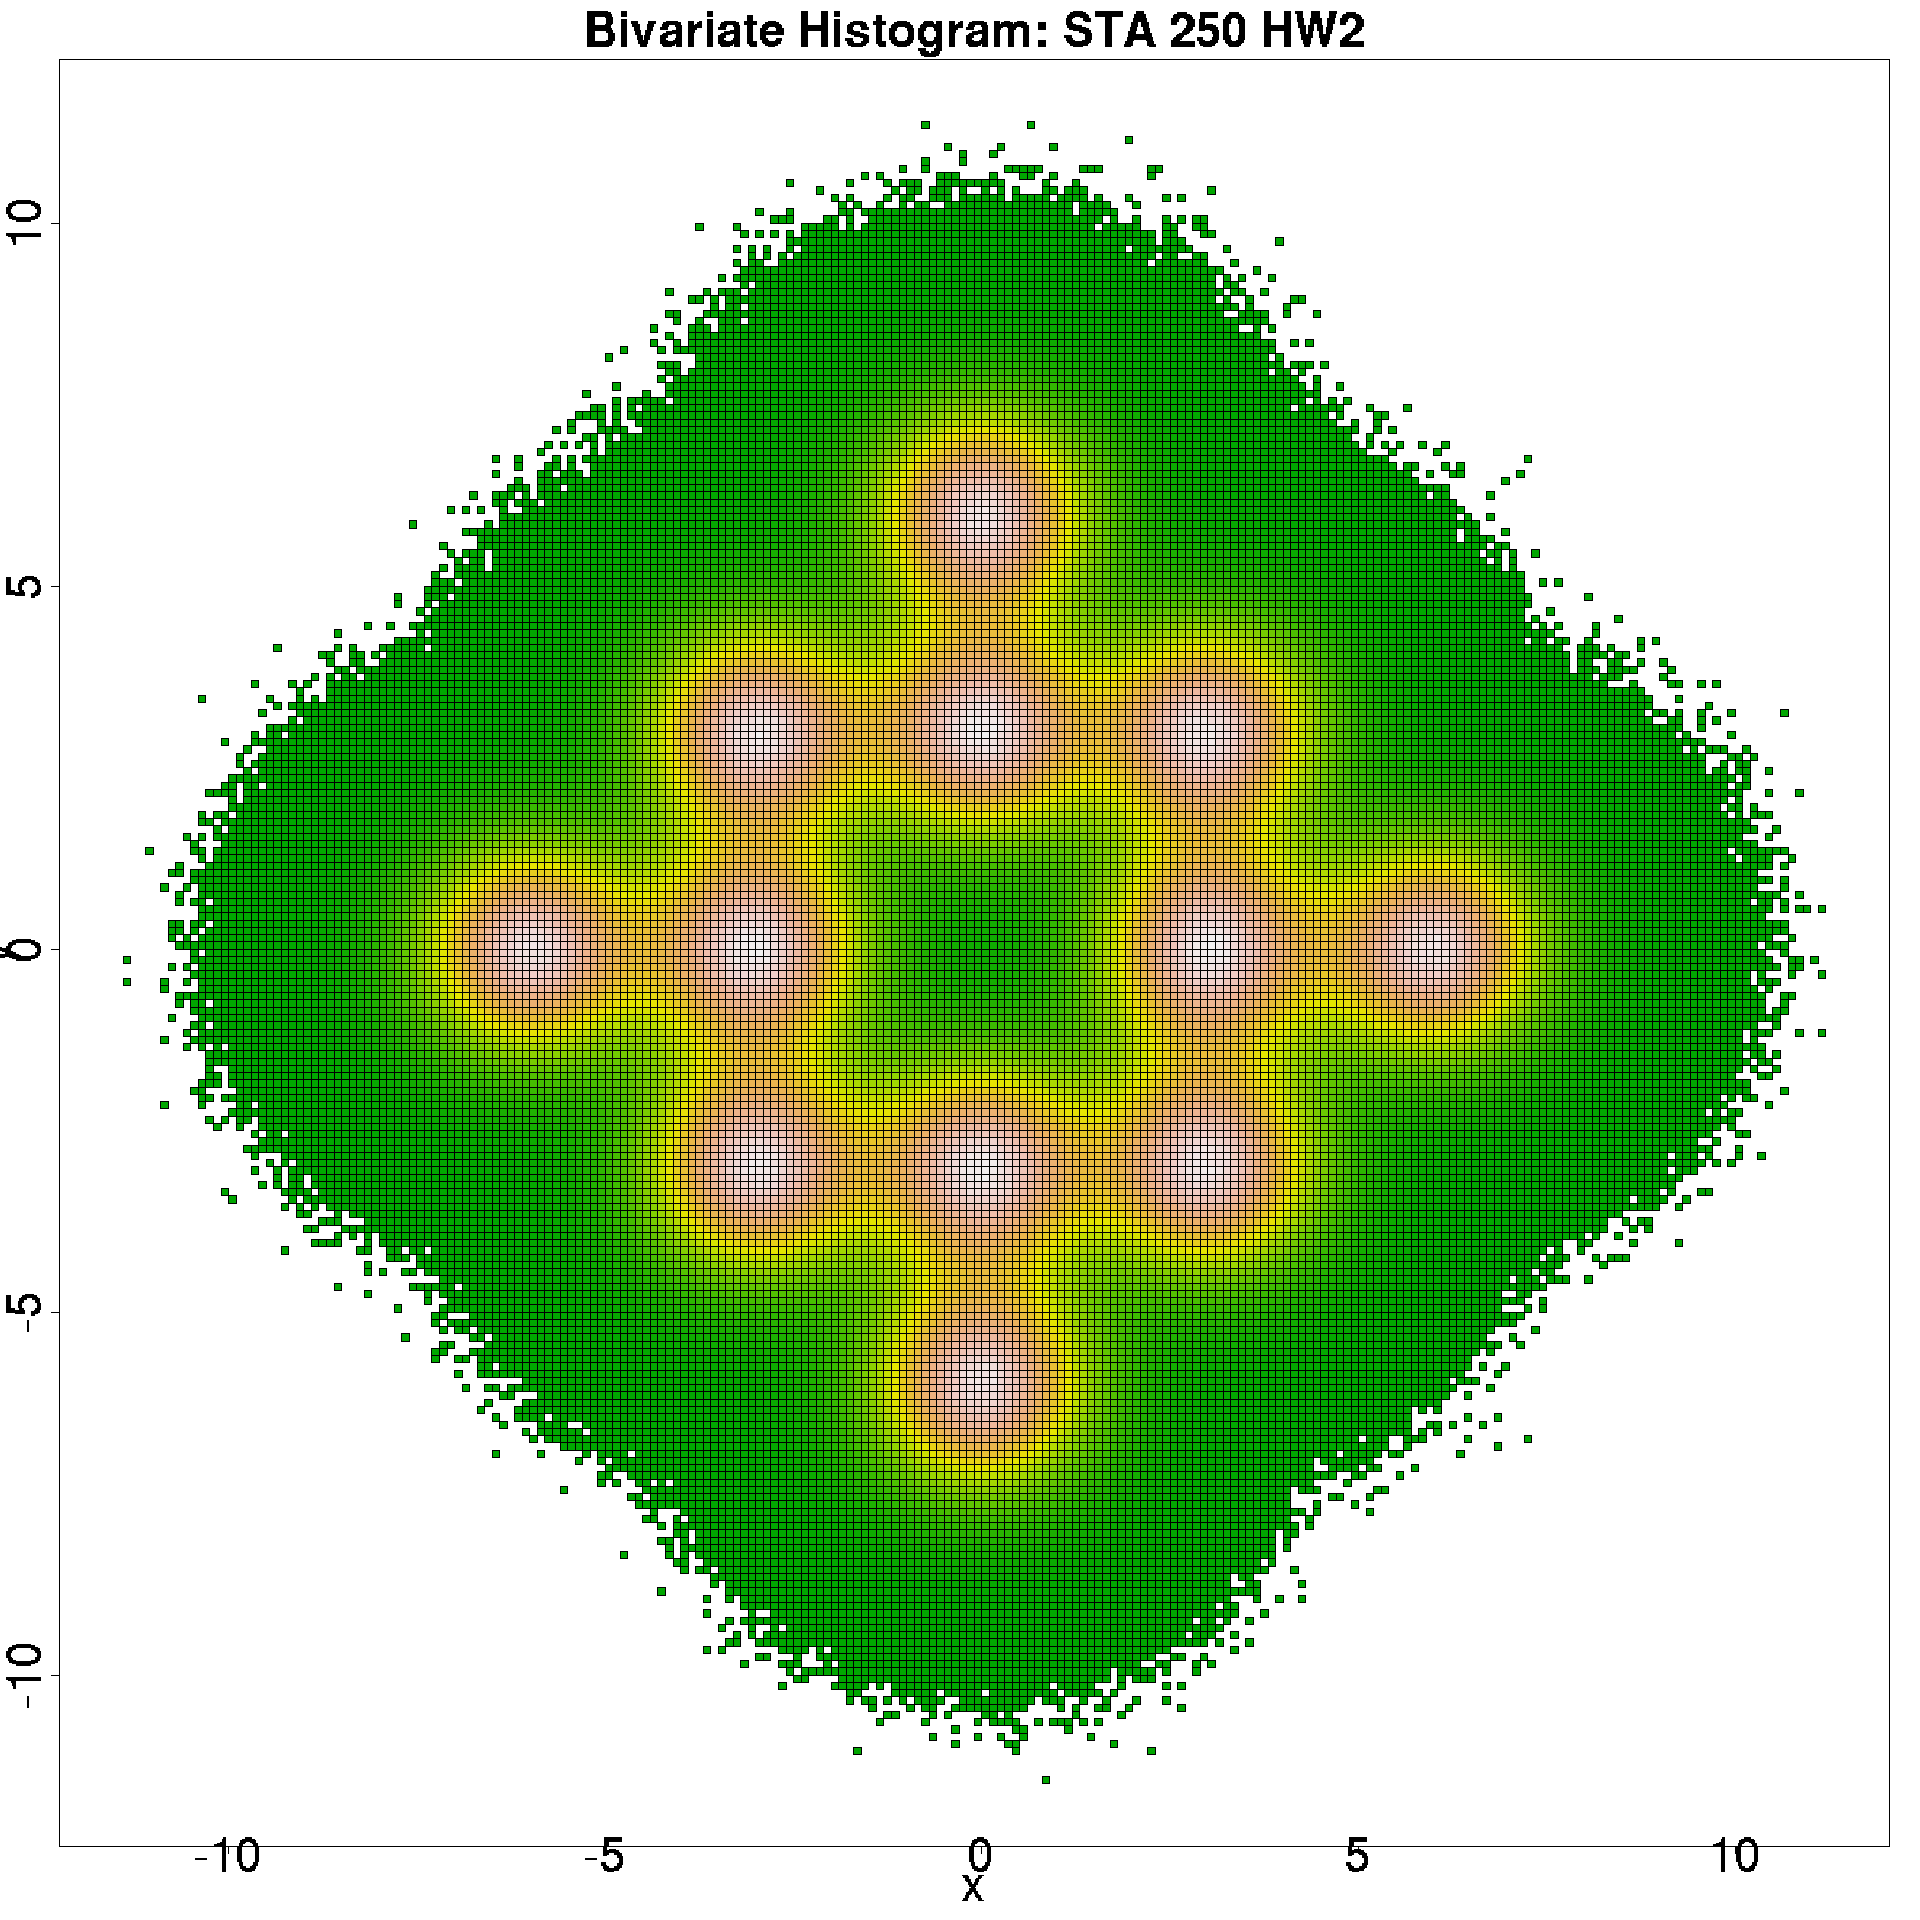
\includegraphics[scale=.15]{Streaming/hist2d.png}
\caption*{Two-dimensional histogram, $n=180,000,000$.}
\end{figure}

\section*{Hive}
MapReduce works pretty well for a lot of problems, but there are definitely declarative languages that, at the expense of flexibility, make coding incredibly easy. One of the easiest languages to write code for is SQL (structured query language). While relational data (tables--the type of data SQL works for) is a restrictive paradigm in some circumstances, it tends to make a lot of sense in statistics. So what happens if we want the scalability of MapReduce with the simplicity of SQL's syntax?

Hive exists as an add-on for Hadoop MapReduce that allows us to write queries that are similar to SQL, and have the computer figure out the best way to write the Mapper and Reducer. The result is the ability to write fairly complicated relations in only a few lines of code that would've taken MapReduce much more grief. In this example, we have data from 1000 different groups (you can think of this as a really big ANOVA, if you'd like). The data is large enough that doing within-group means and variances would be troublesome for R, so we consider using MapReduce. This task is almost a single line for (S)QL to do, so we'd like to leverage some of (S)QL's simplicity. 

The first challenge with Hive is that, like relational databases, we are required to specify the data's schema up front. This is simple enough--we know that the S3-bucketed data is comprised of two tab-delimited columns: an integer representing the group an observation belongs to, and the value of that observation, which we represent in the most precise float Hive allows: a double. Simply specifying the schema is not enough to get our data however--we also need to load it into to our new schema. Because the data was stored as a text file, we cannot take advantage of an external load (which would've saved I/O and space and been impractical for very large datasets), so we copy the data over from the S3 bucket and load with the \verb+LOAD DATA LOCAL+ statement, and point it to the file location. The data is now loaded, so we initialize a new table where we will store the within-group means and variances, both as doubles. For reference, we'll also store the group identifier as well. The reason people love (S)QL so much (myself included), is because the syntax is so powerful that getting the means and variances is as simple as asking to select all means and variances of the values, grouped by the group. As written, that is very nearly correct QL syntax! Refer to the appendix for correct Hive syntax. The final group means and variances was printed to a tab-delimited file (the default), then converted to a comma-separated value file using a Perl/sed one-liner. 

One thing to mention: Hive was very slow, relative to traditional relational databases. One reason this could be the case is that the group index was not an indexed variable. With indexed variables, each record can be accessed in constant time. While I'm guessing that the data is accessed in a way that's faster than O(n), I'm not sure that a naive table initialization as I've done is the most efficient at recalling records by group. Three seconds is not a long time, but I'm sure that with indexing, three seconds would be a signal that something was wrong if the same query was run in Postgres or a similarly modern RDBMS. 207MB of data is tiny.

For future reference, Facebook recently open-sourced the code for a new type of distributed relational language, similar in objective to Hive, yet different in implementation. This new language, Presto, is an order of magnitude faster than Hadoop. This means that even on small datasets like this one, Presto would have performance that would be competitive with RDBMS's, and still allow the data to be stored in a super-distributed fashion. For more information, see the official open-source announcement from November 6, 2013: \url{http://goo.gl/HHaFCH}.

Here is a plot of the group means versus the group variances.
\begin{figure}[H] \center
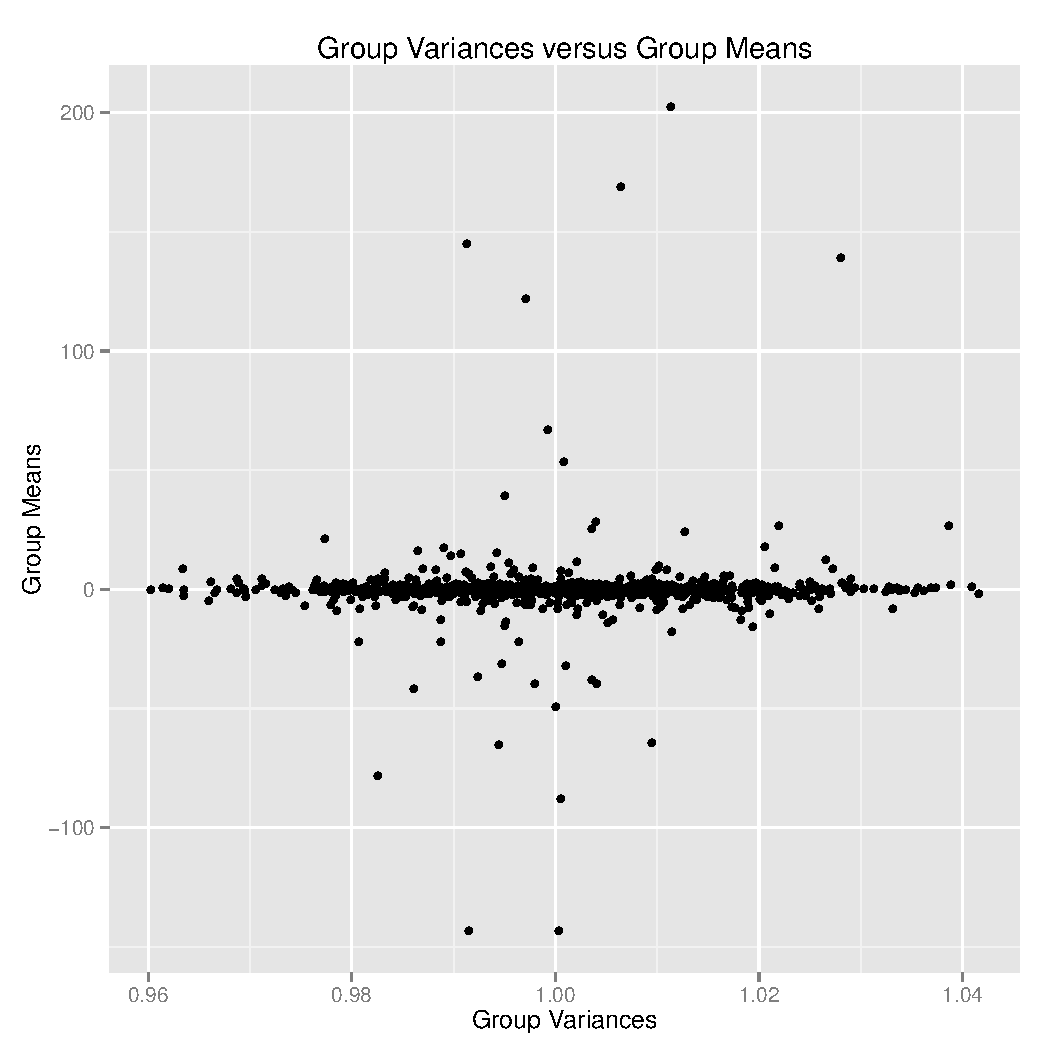
\includegraphics[scale=.75]{Hive/mean_by_var.pdf}
\caption*{Scatterplot of variances versus means for the 1000 groups.}
\end{figure}

\section*{Appendix: R Source Code}
\subsection*{Bag of Little Bootstraps Code:}
BLB\_lin\_reg\_pre.R:
The pre-algorithm file. Sequentially, this file uses the hash table provided by the big matrix to subset the very large dataset in an efficient manner. It then saves each subsetted dataset to an RData file, which can be loaded very easily. The code at the beginning pertaining to fastmatch may be somewhat foreign. It will determine if the current system has fastmatch install. If it does not, it will attempt to download the fastmatch package from the Berkeley CRAN mirror.
\lstinputlisting{"BLB/BLB_lin_reg_pre.R"}

BLB\_lin\_reg\_job.R:
The file distributed to the nodes on the cluster. It takes in the correct subset of the big dataset, simulates the counts of each unique value, runs a linear model to get coefficients, then returns those coefficients to a unique file.
\lstinputlisting{"BLB/BLB_lin_reg_job.R"}

BLB\_lin\_reg\_process.R:
Process will handle joining all the unique files back together, taking the averages over the bootstraps, then getting a single estimate of standard error for each covariate. Creates a plot of the standard error versus the covariate position.
\lstinputlisting{"BLB/BLB_lin_reg_process.R"}

\newpage
\subsection*{MapReduce Code:}
Mapper.py:
Takes lines of $(X,Y)$ pairs from STDIN, creates bins for each pair, then outputs the corresponding bins as a list, tabbed-separated from the count of pairs on each line ($1$ in every case), to STDOUT.
\lstinputlisting[language=Python]{Streaming/mapper.py}

Reducer.py:
Takes sorted key-value pairs (strings separated by tabs), counts the number of times each key is seen, then outputs the bins and count to STDOUT, comma separated.
\lstinputlisting[language=Python]{Streaming/reducer.py}

\newpage
\subsection*{Hive Code:}
get\_group\_means.sh:
Reads the data (assuming the data is stored in a folder under the user's home called hive\_data, in a file called groups.txt) in to Hive, runs a QL script, outputs all the group means and variances to a file, then runs a Perl script to convert tab-delimiting into comma-delimiting.
\lstinputlisting[language=bash]{Hive/get_group_means.sh}

t\_hive.sql:
Not really a SQL script, true, but very similar. Declare input data schema, then import the data from a text file. From that data, declare a new schema which stores the group means and variances, and compute them. 
\lstinputlisting[language=SQL]{Hive/t_hive.sql}
\end{document} 